\documentclass[11pt]{article}
\usepackage[margin=1in]{geometry}
\usepackage{amsmath,amssymb}
\usepackage{graphicx}
\usepackage{booktabs}
\usepackage[colorlinks=true,linkcolor=blue,citecolor=blue,urlcolor=blue]{hyperref}

% --- the only two lines to edit before submission ---
\newcommand{\authorname}{Singularity}
\newcommand{\affiliation}{}

\title{Oversampling rare failures: what SMOTE does to surrogate-based\\ failure probabilities}
\author{\authorname\\ \small \affiliation}
\date{\today}

\begin{document}
\maketitle

\begin{abstract}
Classifiers are increasingly used as surrogates of limit-state functions in structural reliability, and because
failures are rare they are often trained on data rebalanced with the synthetic minority oversampling technique
(SMOTE). Its effect on the estimated failure probability $P_f$ has not, to our knowledge, been measured. We compare,
on three standard benchmarks (a four-branch series system, a non-linear oscillator and a ten-variable linear limit
state), a classifier trained on plain Monte Carlo samples, class weighting, SMOTE, and SMOTE followed by a Bayes
prior-shift correction, with gradient boosting and a neural network, 50 repetitions each and 2000 training points.
The direction of the error depends on how many failures the training sample contains. With about nine failures
(four-branch, $P_f=4.4\times10^{-3}$) SMOTE overestimates $P_f$ by a median factor of 11--13; the correction reduces
this to 0.6--2.4. With about 57 failures (oscillator) all strategies are within a factor 0.7--1.2. With about three
failures (linear, $P_f=1.35\times10^{-3}$) the plain classifier collapses to medians of 0.00--0.03 of the true value,
SMOTE recovers 0.6--0.7 but with a 10--90\% range of 0.12--1.96, and the correction collapses again. No strategy is
safe across regimes: a thresholded classifier, rebalanced or not, should not be used as a failure-probability
estimator without a check against the true limit state.
\end{abstract}

\section{Introduction}
Surrogate models make reliability analysis affordable when each evaluation of the limit-state function $g$ is
expensive~\cite{Sudret}. Classification surrogates predict the sign of $g$, and the failure probability is estimated
by applying the classifier to a large Monte Carlo sample. Because failures are rare, the training data are
imbalanced, and rebalancing with SMOTE~\cite{Chawla} has been proposed to help the surrogate learn the failure region,
for example in ship-structure design~\cite{Ship}. In risk prediction for medicine, rebalancing is known to miscalibrate
predicted probabilities~\cite{vandenGoorbergh}. Whether the same happens to $P_f$ in reliability analysis, and in
which direction, is the question of this note. It was prompted by an automated forecast that SMOTE would enter
computational mechanics.

\section{Methods}
\paragraph{Benchmarks} (standard normal inputs).
\begin{itemize}
\item Four-branch series system~\cite{Waarts}, 2 variables, $k=6$: $P_f=4.44\times10^{-3}$ (from $10^6$ samples).
\item Non-linear undamped oscillator, 6 variables, with the usual parameter distributions: $P_f=2.85\times10^{-2}$.
\item Linear limit state $g=3\sqrt{10}-\sum_{i=1}^{10}x_i$: $P_f=\Phi(-3)=1.35\times10^{-3}$ exactly.
\end{itemize}
\paragraph{Strategies.} A classifier is trained on 2000 Monte Carlo points labelled by the sign of $g$:
(i) plain; (ii) class weights inversely proportional to class frequency (gradient boosting only); (iii) SMOTE to a
balanced sample ($k=5$); (iv) SMOTE followed by the prior-shift correction
$p'=\dfrac{p\,\hat\pi/\pi_s}{p\,\hat\pi/\pi_s+(1-p)(1-\hat\pi)/(1-\pi_s)}$, where $\pi_s=0.5$ is the balanced
prevalence and $\hat\pi$ the failure share in the training sample. $P_f$ is estimated as the share of $2\times10^5$
new points classified as failures ($p>0.5$).
\paragraph{Classifiers.} Histogram gradient boosting (200 iterations) and a two-layer perceptron (32--32).
\paragraph{Protocol.} 50 repetitions per configuration; repetitions with fewer than two failures in the training
sample are skipped and counted (13--14 of 50 for the linear case). Everything was fixed before the single run.

\section{Results}
\begin{figure}[t]
\centering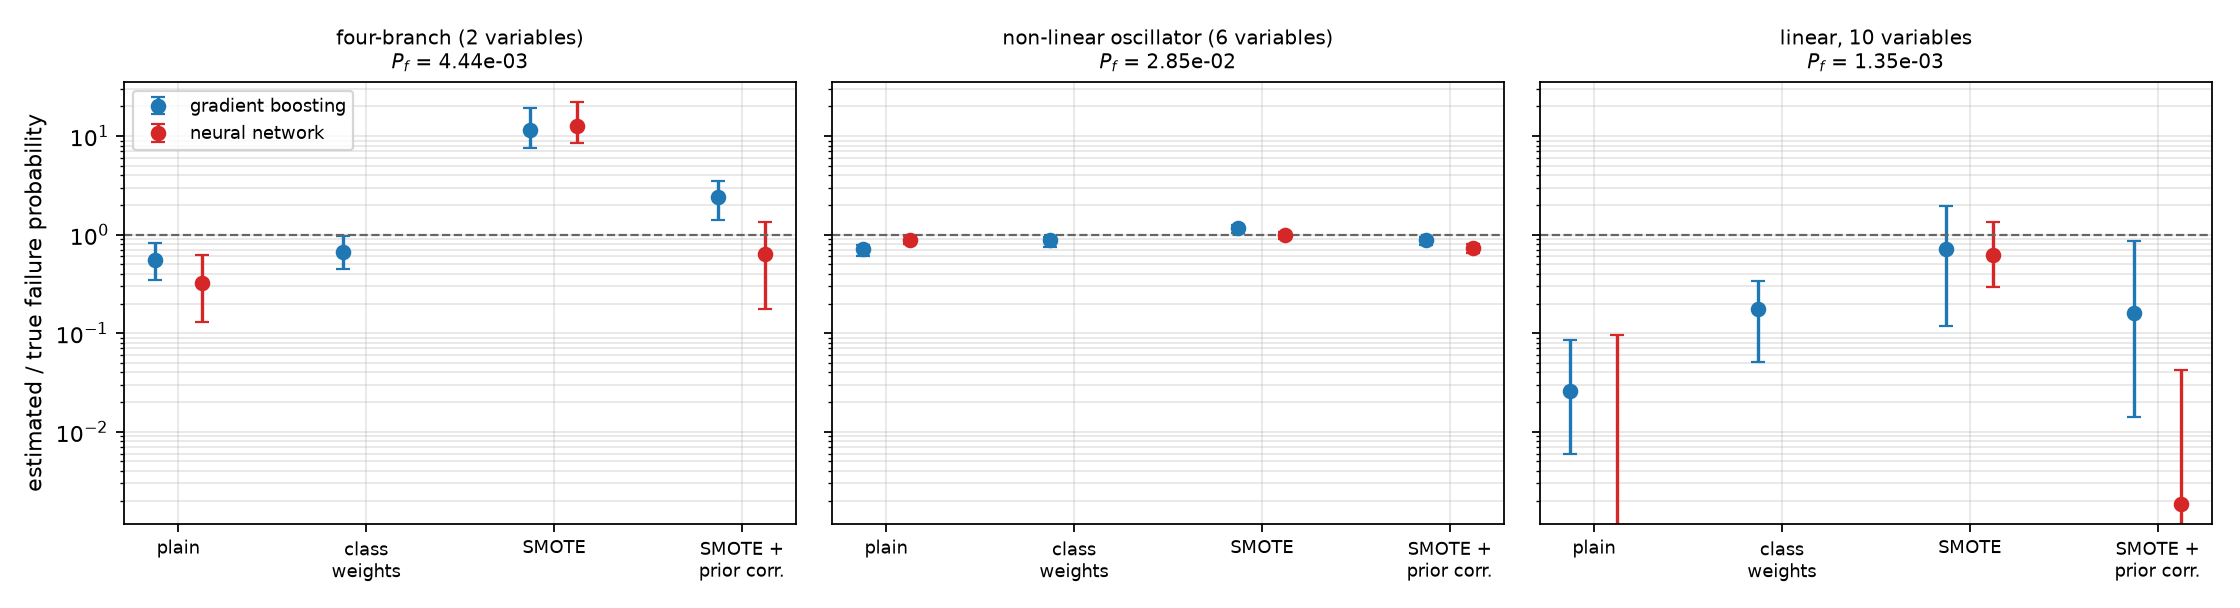
\includegraphics[width=\linewidth]{fig_bias.png}
\caption{Estimated over true failure probability: median and 10--90\% range over repetitions (log scale).}
\label{fig}
\end{figure}

\begin{table}[h]
\centering
\begin{tabular}{llcccc}
\toprule
benchmark & classifier & plain & class weights & SMOTE & SMOTE + correction \\
\midrule
four-branch & boosting & 0.56 & 0.67 & 11.4 & 2.39 \\
 & neural net & 0.32 & -- & 12.8 & 0.63 \\
oscillator & boosting & 0.72 & 0.88 & 1.17 & 0.88 \\
 & neural net & 0.88 & -- & 0.99 & 0.74 \\
linear, 10 variables & boosting & 0.03 & 0.17 & 0.71 & 0.16 \\
 & neural net & 0.00 & -- & 0.63 & 0.00 \\
\bottomrule
\end{tabular}
\caption{Median ratio of estimated to true $P_f$.}
\label{tab}
\end{table}

Three regimes appear (Figure~\ref{fig}, Table~\ref{tab}).
\begin{itemize}
\item \textbf{Few but informative failures} (four-branch, about 9 in the training sample): the plain classifier
underestimates (0.3--0.6), SMOTE overestimates by an order of magnitude, the correction brings the estimate back
within a factor 2.5.
\item \textbf{Many failures} (oscillator, about 57): every strategy is within a factor 0.7--1.2; SMOTE is the closest.
\item \textbf{Very few failures} (linear, about 3): the plain classifier predicts almost no failures; SMOTE is the
only strategy near the true value, but with a spread of more than an order of magnitude; the correction undoes it.
\end{itemize}
SMOTE always raises recall (for example from 0.35 to 0.73 on the four-branch system), which is why it is attractive;
but recall is not the quantity a reliability analysis needs.

\section{Discussion}
SMOTE moves the decision boundary toward the safe region. Whether this corrects or creates bias depends on how far
the plain classifier was from the true boundary, which is unknown in practice. The prior-shift correction is exact for
calibrated probabilities but cannot fix a boundary that was never learnt. The practical rule is therefore negative but
useful: report a classifier-based $P_f$ only together with a check against the true limit state --- for example
evaluating $g$ on the points the surrogate classifies as failures, or using the surrogate only to build an importance
sampling density --- and prefer adaptive designs that place training points near the boundary.

\paragraph{Limitations.} Three benchmarks, one training size, two classifiers, a 0.5 threshold; adaptive (active
learning) surrogates, which are the state of the art, are not compared.

\paragraph{Reproducibility.} \texttt{experiment.py} regenerates every number and the figure.

\paragraph{Origin of the question.} The question came from an automated forecast (Singularity v3, registered on 5
November 2026 with a SHA-256 fingerprint, view without generative AI) that SMOTE would enter the subfield
\emph{Computational Mechanics}. The forecast concerned the arrival of the method, not the result of this note.

\begin{thebibliography}{9}
\bibitem{Sudret} B.~Sudret, Meta-models for structural reliability and uncertainty quantification, arXiv:1203.2062 (2012).
\bibitem{Chawla} N.~V.~Chawla et al., SMOTE: synthetic minority over-sampling technique, \emph{JAIR} 16 (2002) 321--357.
\bibitem{Ship} SMOTE-assisted surrogate for ship-structure reliability-based design optimization, \emph{Chinese Journal of Ship Research}, doi:10.19693/j.issn.1673-3185.01657.
\bibitem{vandenGoorbergh} R.~van den Goorbergh et al., The harm of class imbalance corrections for risk prediction models, \emph{JAMIA} 29 (2022) 1525--1534.
\bibitem{Waarts} P.~H.~Waarts, \emph{Structural reliability using finite element analysis}, PhD thesis, TU Delft (2000).
\end{thebibliography}
\end{document}
